\documentclass[a4paper]{article}
\usepackage[a4paper, total={6in, 8in}]{geometry}
\usepackage[english]{babel}
\usepackage[utf8]{inputenc} 
\usepackage{amsmath,amssymb}
\usepackage{parskip} 
\usepackage[usenames,dvipsnames,table]{xcolor} 
\usepackage{fancyvrb} 
\PassOptionsToPackage{hyphens}{url}\usepackage{hyperref} 
\DeclareMathOperator{\E}{\mathbb{E}}
\usepackage{amsthm}
\newtheorem{theorem}{Theorem}
\usepackage{mdframed}
\usepackage{xcolor}
\usepackage{framed}
\usepackage{listings}
\usepackage{graphicx} % Allows including images
\usepackage{booktabs} % Allows the use of \toprule, \midrule and \bottomrule in tables
\usepackage{amsmath,amssymb}
\usepackage{tikz}
\usetikzlibrary{arrows}
\usepackage{mathtools}
\usepackage{float}
\usepackage{fancyvrb} 
\usepackage{pgfplots}
\pgfplotsset{compat=newest}
%% the following commands are needed for some matlab2tikz features
\usetikzlibrary{plotmarks}
\usetikzlibrary{arrows.meta}
\usepgfplotslibrary{patchplots}
\usepackage{grffile}
\usepackage{bm}
\usepackage{amsmath}
\usetikzlibrary{patterns}
\usepackage{subcaption}
\usepackage{rotating}
\usepackage{lscape}
\usepackage{standalone}
\usepackage{enumitem}
\usepackage{threeparttable}
\usepackage{shadethm}
\usepackage{setspace}
\usepackage{centernot}
\usepackage{adjustbox}
\usetikzlibrary{calc,matrix}
\newshadetheorem{thm}{Theorem}
\definecolor{shadethmcolor}{HTML}{EDF8FF}
\definecolor{shaderulecolor}{HTML}{45CFFF}
\setlength{\shadeboxrule}{.4pt}
\setlength{\parindent}{5ex}
\usepackage[section]{placeins}

\makeatletter
\@addtoreset{equation}{section}
\@addtoreset{equation}{subsection}
\@addtoreset{equation}{subsubsection}
\@addtoreset{equation}{paragraph}
\@addtoreset{equation}{subparagraph}
\makeatother


\hypersetup{
	colorlinks = true,
	urlcolor   = blue,
	linkcolor  = blue,
	citecolor  = red
}

\usepackage{logicproof} 
\usepackage{tikz} 
\usetikzlibrary{trees,positioning}
\usepackage{tikz}


\DeclareMathOperator{\di}{d\!}
\newcommand*\Eval[3]{\left.#1\right\rvert_{#2}^{#3}}


% ------------------------------------------------------------------------------------
% ------------------------------------------------------------------------------------



\title{}
\author{Problem Set IV -  Sharp Regression Discontinuity\\
	\small{\emph{Enrijeta Shino}}}


\begin{document}
	\maketitle



\section{ (Sharp) Regression Discontinuity}

\noindent \textbf{Framework}

\noindent The dataset that I use in this part is the smoking data. The cut-off point is the $age = 45$ and I create a placebo treatment by applying the following rule: 

\noindent \textbf{Decision rule:} 

\noindent Let $\tilde{Y} = \text{consumption of cigarettes}$ and $C = \text{age of consumers}$. 

\begin{equation} \tilde{Y}_i = 
\begin{cases}
	\tilde{Y}_i(0) & if \quad c > 45 \\
	\tilde{Y}_i(1) & otherwise
\end{cases}
\end{equation}

\noindent where we manipulate the outcome $Y$ to create the sharp discontinuity design framework. We assume that consumers above the age of $45$ receive a treatment in order to reduce consumption of cigarettes. 

\noindent\textbf{Randomly generated outcomes:}

\noindent We create the outcomes $(\tilde{Y}_i(1), \tilde{Y}_i(0))$ as follows: 

\begin{align}
\tilde{Y}_i(1)  &= Y_i + \sigma_{Y_i} + \epsilon_i \\
\tilde{Y}_i(0) &=  Y_i + \sigma_{Y_i} + \eta_i 
\end{align}

where $\epsilon_i \sim U(0,1)$ and $\eta_i \sim U(0,1)$ are both randomly generated numbers in R. 

\noindent\textbf{Testing and visual inspection:}

\noindent We apply McCrary (2008)  to test whether the discontinuity in the density of the running variable (age) at the cut-off point (age = 45) is equal to zero. The p-value is equal to $0.0077$, hence we reject the null hypothesis. 

\begin{figure}[!htb]
	\centering
	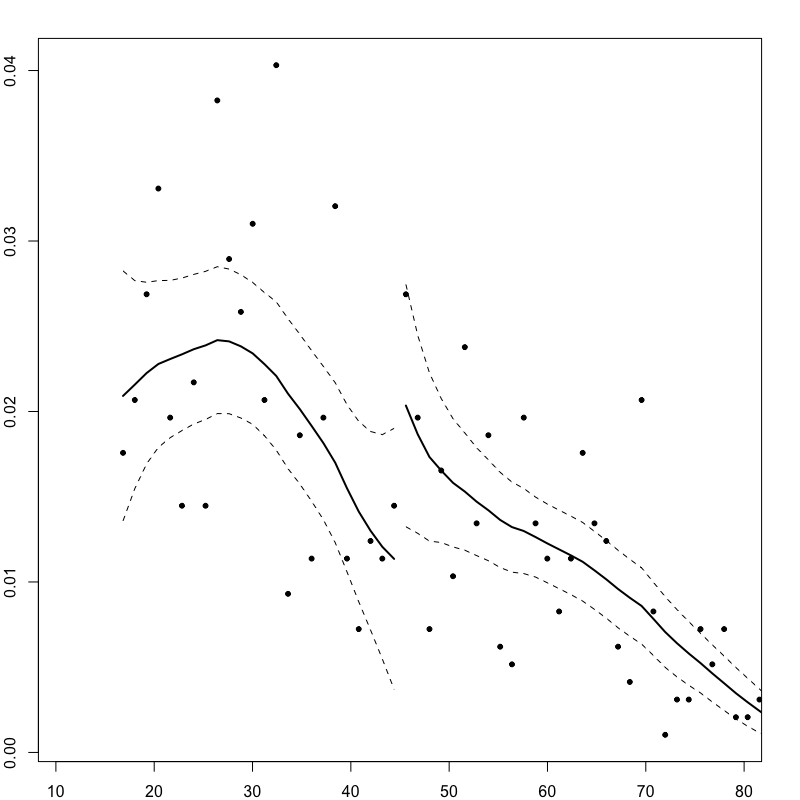
\includegraphics[width=0.6\textwidth]{Rplot1.png}
	\captionof{figure}{McCrary (2008) test}
\end{figure}

\pagebreak

\noindent \textbf{2.1 Plot the outcome by forcing variable (the standard graph showing the discontinuity)}


\begin{figure}[!htb]
	\centering
	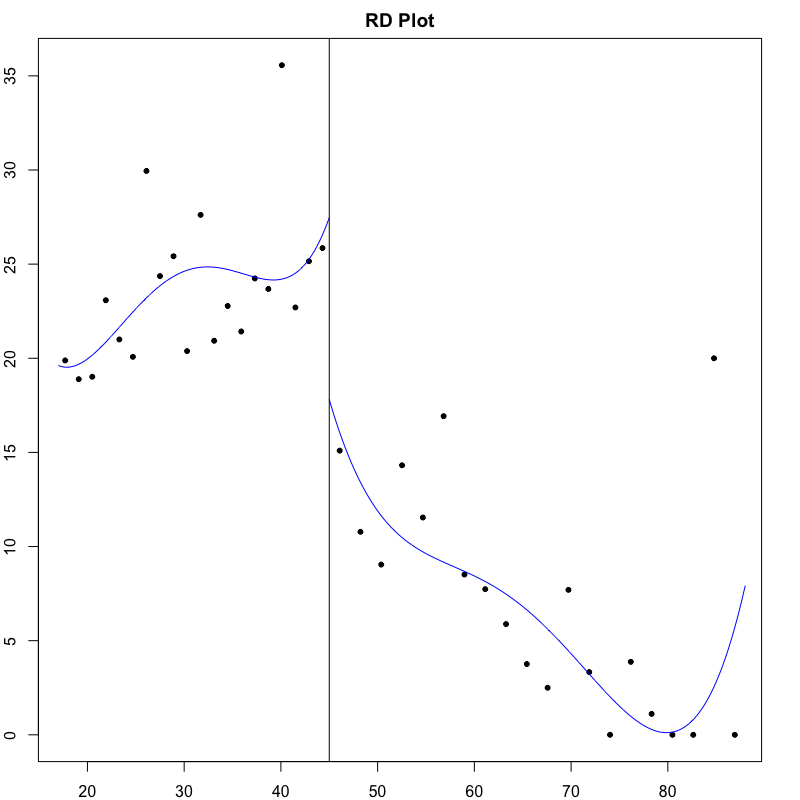
\includegraphics[width=0.6\textwidth]{Rplot2.png}
	\captionof{figure}{Consumption of cigarettes by age}
\end{figure}

\pagebreak
\noindent\textbf{2.2. Plot the density of the forcing variable}

\begin{figure}[!htb]
	\centering
		\centering
		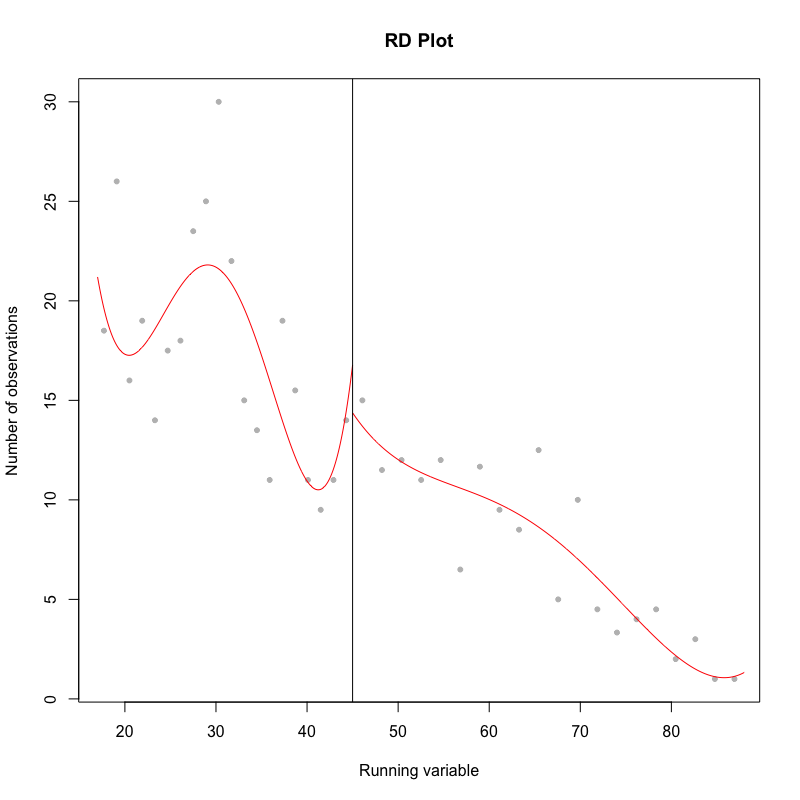
\includegraphics[width=.8\linewidth]{Rplot3.png}
		\captionof{figure}{Density of the Forcing Variable}
		\label{fig:test1}
\end{figure}

\begin{figure}[!htb]
		\centering
		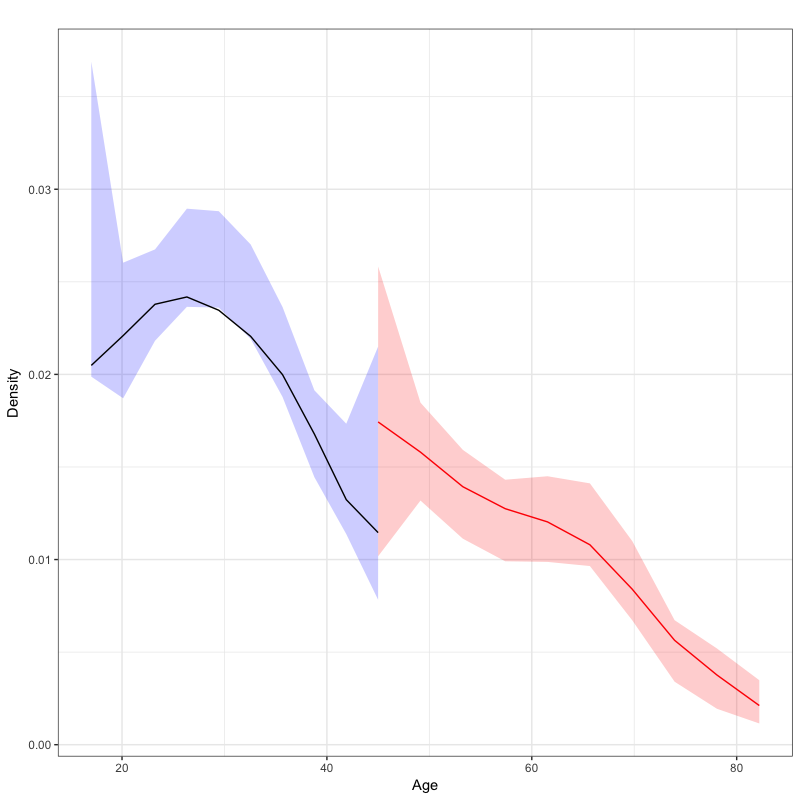
\includegraphics[width=0.8\linewidth]{Rplot4.png}
		\captionof{figure}{Density of the Forcing Variable}
		\label{fig:test2}
\end{figure}

\begin{figure}[!htb]
	\centering
	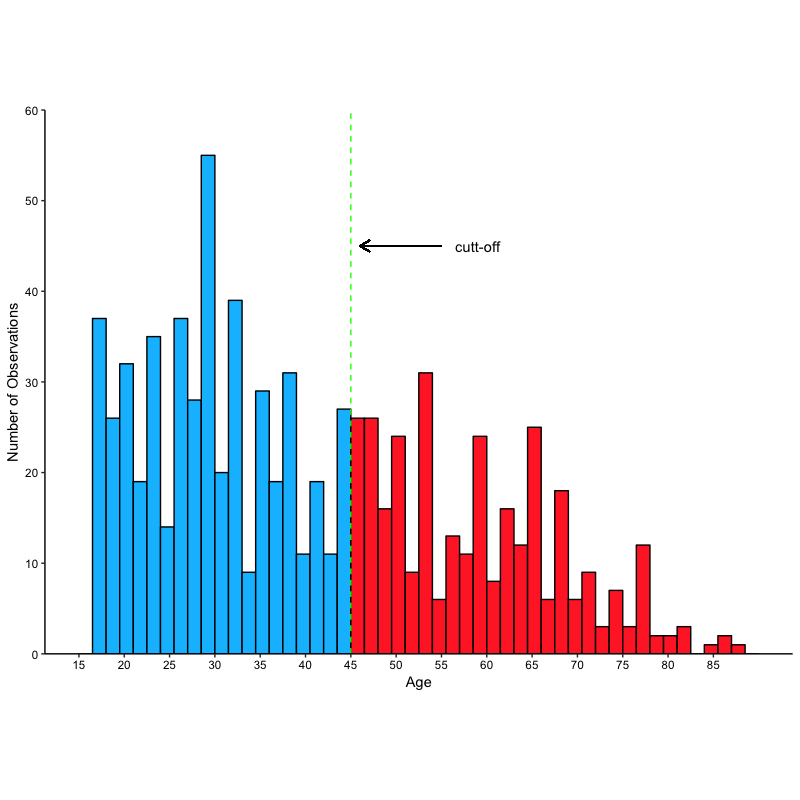
\includegraphics[width=1\textwidth]{Rplot5.png}
	\captionof{figure}{Distribution of the Forcing Variable (Not Sorted)}
\end{figure}

\begin{figure}[!htb]
	\centering
	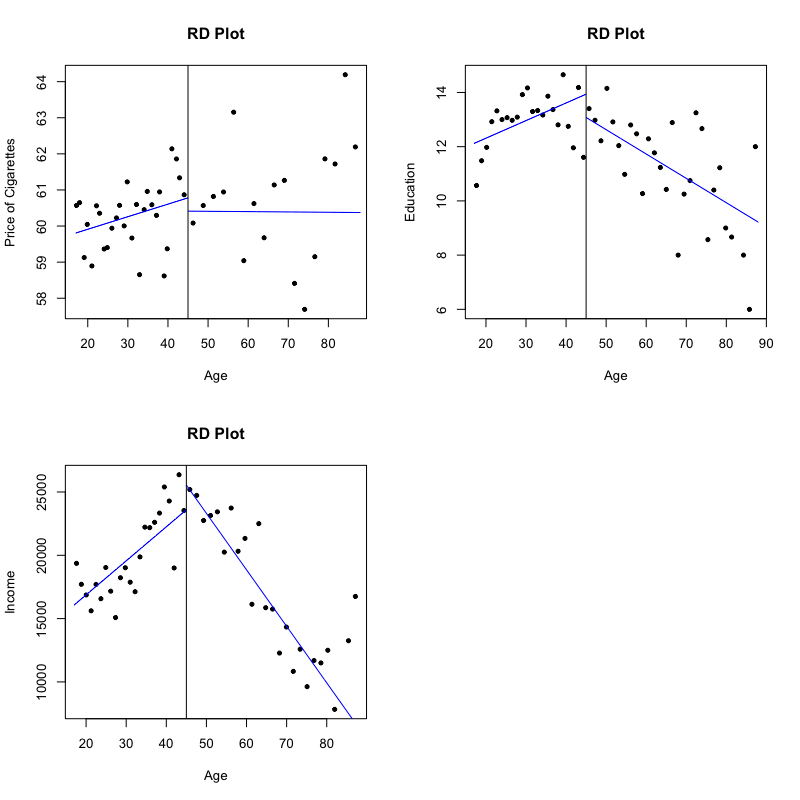
\includegraphics[width=1\textwidth]{Rplot6.png}
	\captionof{figure}{Continuity of covariates}
\end{figure}

\FloatBarrier

\noindent \textbf{2.3. Estimate the effect using a local linear regression}

\begin{itemize}
	\item Local linear regression using a uniform kernel 
\end{itemize}



\begin{table}[ht!]
		\caption{\textbf{RDD results for local linear regression (using the package \& uniform kernel)}} 
	\begin{center}
			\begin{threeparttable}
				\begin{tabular}{lccccc}
					\hline
					Method & Coef. & Std. Err. & z & p-value & 95\% C.I. \\
					\hline
					Convential & \textbf{-5.580} & 5.946  & -0.938 & 0.348  & [-17.234 , 6.074] \\
					Robust & & & -0.486 &  0.627 &  [-16.573 , 9.985]  \\
					\hline
				\end{tabular}
				\end{threeparttable}
		\end{center}
	\end{table}

\begin{table}[!htbp] \centering 
	\caption{RDD results for local linear regression (uniform kernel)} 
	\label{} 
	\begin{tabular}{@{\extracolsep{5pt}}lcc} 
		\\[-1.8ex]\hline 
		\hline \\[-1.8ex] 
		& \multicolumn{2}{c}{\textit{Dependent variable:}} \\ 
		\cline{2-3} 
		\\[-1.8ex] & \multicolumn{2}{c}{cigs\_new} \\ 
		\\[-1.8ex] & (LHS) & (RHS)\\ 
		\hline \\[-1.8ex] 
		I(age - 45) & $-$0.232 & $-$2.251$^{**}$ \\ 
		& (1.182) & (0.887) \\ 
		& & \\ 
		Constant & \textbf{24.600}$^{***}$ & \textbf{19.020}$^{***}$ \\ 
		& (4.579) & (3.151) \\ 
		& & \\ 
		\hline \\[-1.8ex] 
		Observations & 68 & 92 \\ 
		R$^{2}$ & 0.001 & 0.067 \\ 
		Adjusted R$^{2}$ & $-$0.015 & 0.056 \\ 
		Residual Std. Error & 17.632 (df = 66) & 17.047 (df = 90) \\ 
		F Statistic & 0.038 (df = 1; 66) & 6.443$^{**}$ (df = 1; 90) \\ 
		\hline 
		\hline \\[-1.8ex] 
		\textit{Note:}  & \multicolumn{2}{r}{$^{*}$p$<$0.1; $^{**}$p$<$0.05; $^{***}$p$<$0.01} \\ 
	\end{tabular} 
\end{table} 

\begin{equation}
\text{\textbf{ATE}} = 19.02 - 24.6 = \textbf{-5.58}
\end{equation}

\textbf{2.4. Estimate the effect using a local polynomial (of order 2 and 3) regression}

\begin{itemize}
	\item  \textbf{2nd order local polynomial regression }
\end{itemize}

\begin{table}[ht!]
	\caption{\textbf{RDD results for 2nd order local polynomial regression (using the package \& uniform kernel)}} 
	\begin{center}
		\begin{threeparttable}
			\begin{tabular}{lccccc}
				\hline
				Method & Coef. & Std. Err. & z & p-value & 95\% C.I. \\
				\hline
				Conventional  & \textbf{3.495}  & 8.716  & 0.401  & 0.688  &  [-13.589 , 20.578]    \\
				Robust      &           &    & 0.584 &    0.559 &  [-12.988 , 24.019]    \\
				\hline
			\end{tabular}
		\end{threeparttable}
	\end{center}
\end{table}

\begin{table}[!htbp] \centering 
	\caption{RDD results for 2nd order local polynomial regression (uniform kernel)} 
	\label{} 
	\begin{tabular}{@{\extracolsep{5pt}}lcc} 
		\\[-1.8ex]\hline 
		\hline \\[-1.8ex] 
		& \multicolumn{2}{c}{\textit{Dependent variable:}} \\ 
		\cline{2-3} 
		\\[-1.8ex] & \multicolumn{2}{c}{cigs\_new} \\ 
		\\[-1.8ex] & (LHS) & (RHS)\\ 
		\hline \\[-1.8ex] 
		I(age - 45) & $-$1.346 & $-$11.030$^{***}$ \\ 
		& (4.383) & (2.611) \\ 
		& & \\ 
		I((age - 45)$\hat{\mkern6mu}$2) & $-$0.142 & 1.445$^{***}$ \\ 
		& (0.529) & (0.367) \\ 
		& & \\ 
		Constant & \textbf{23.023}$^{***}$ & \textbf{26.518}$^{***}$ \\ 
		& (7.434) & (3.762) \\ 
		& & \\ 
		\hline \\[-1.8ex] 
		Observations & 86 & 101 \\ 
		R$^{2}$ & 0.001 & 0.156 \\ 
		Adjusted R$^{2}$ & $-$0.023 & 0.138 \\ 
		Residual Std. Error & 17.265 (df = 83) & 16.104 (df = 98) \\ 
		F Statistic & 0.061 (df = 2; 83) & 9.027$^{***}$ (df = 2; 98) \\ 
		\hline 
		\hline \\[-1.8ex] 
		\textit{Note:}  & \multicolumn{2}{r}{$^{*}$p$<$0.1; $^{**}$p$<$0.05; $^{***}$p$<$0.01} \\ 
	\end{tabular} 
\end{table} 

\vspace{5cm}

\begin{equation}
\text{\textbf{ATE}} = 26.518 - 23.023 = \textbf{3.495}
\end{equation}



\begin{itemize}
	\item  \textbf{3rd order local polynomial regression }
\end{itemize}

\begin{table}[ht!]
	\caption{\textbf{RDD results for 3nd order local polynomial regression (using the package \& uniform kernel)}} 
	\begin{center}
		\begin{threeparttable}
			\begin{tabular}{lccccc}
				\hline
				Method & Coef. & Std. Err. & z & p-value & 95\% C.I. \\
				\hline
				Conventional   &  \textbf{3.766}   &  9.546   &  0.395  &   0.693   & [-14.944 , 22.476]    \\
				Robust         &         & &     0.484  &   0.629 &  [-15.020 , 24.861]    \\
				\hline
			\end{tabular}
		\end{threeparttable}
	\end{center}
\end{table}

\vspace{6cm}

\begin{table}[!htbp] \centering 
	\caption{RDD results for 2nd order local polynomial regression (uniform kernel)} 
	\label{} 
	\begin{tabular}{@{\extracolsep{5pt}}lcc} 
		\\[-1.8ex]\hline 
		\hline \\[-1.8ex] 
		& \multicolumn{2}{c}{\textit{Dependent variable:}} \\ 
		\cline{2-3} 
		\\[-1.8ex] & \multicolumn{2}{c}{cigs\_new} \\ 
		\\[-1.8ex] & (LHS) & (RHS)\\ 
		\hline \\[-1.8ex] 
		I(age - 45) & $-$2.035 & $-$11.231$^{***}$ \\ 
		& (5.740) & (3.319) \\ 
		& & \\ 
		I((age - 45)$\hat{\mkern6mu}$2) & $-$0.334 & 1.941$^{**}$ \\ 
		& (1.093) & (0.745) \\ 
		& & \\ 
		I((age - 45)$\hat{\mkern6mu}$3) & $-$0.013 & $-$0.091$^{*}$ \\ 
		& (0.060) & (0.046) \\ 
		& & \\ 
		Constant & \textbf{22.496} $^{***}$ & \textbf{26.262}$^{***}$ \\ 
		& (8.007) & (3.879) \\ 
		& & \\ 
		\hline \\[-1.8ex] 
		Observations & 143 & 143 \\ 
		R$^{2}$ & 0.006 & 0.108 \\ 
		Adjusted R$^{2}$ & $-$0.016 & 0.089 \\ 
		Residual Std. Error (df = 139) & 16.181 & 16.002 \\ 
		F Statistic (df = 3; 139) & 0.269 & 5.613$^{***}$ \\ 
		\hline 
		\hline \\[-1.8ex] 
		\textit{Note:}  & \multicolumn{2}{r}{$^{*}$p$<$0.1; $^{**}$p$<$0.05; $^{***}$p$<$0.01} \\ 
	\end{tabular} 
\end{table} 


\begin{equation}
\text{\textbf{ATE}} = 26.262 - 22.496 = \textbf{3.766}
\end{equation}

\noindent Bandwidth is computed using Imbens-Kalyanaraman Optimal Bandwidth and using different kernels: 

\begin{table}[ht!]\centering
	\caption{Bandwidths under different kernels using Imbens-Kalyanaraman Optimal Bandwidth}
	\begin{tabular}{lcccc}
		\hline
	& Rectangular & Triangular & Epanechnikov & Quatric \\
	Bandwidth & 10.23 & 6.51 & 6.51 & 6.92 \\ 	 
	\hline
	\end{tabular}
\end{table}

\begin{table}[ht!]\centering
	\caption{Compare}
	\begin{tabular}{lcccc}
		\hline
		Estimate & Rectangular & Triangular & Epanechnikov & Quatric \\
		\hline
		ATE (local linear)& -10.62 & -5.58 & -5.58 & -5.58 \\
		ATE (local 2nd order poly)& -1.62 & 4.62 &  4.62 & 4.62 \\
		ATE (local 3rd order poly )& 5.05 & -19.33 & -19.33 & -19.32 \\
		\hline
	\end{tabular}
\end{table}


\begin{figure}[!htb]
	\centering
	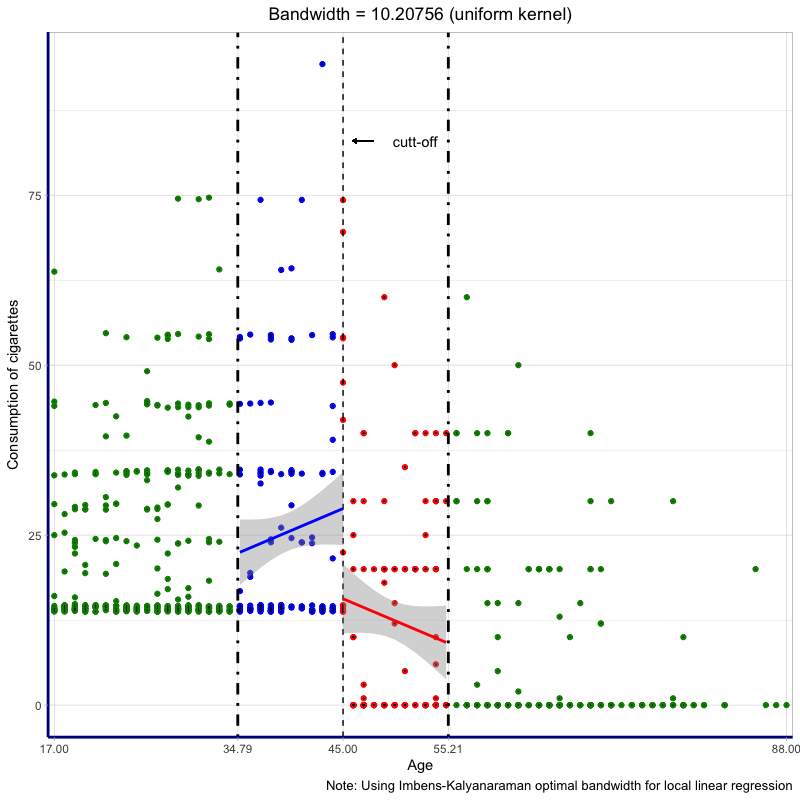
\includegraphics[width=0.99\textwidth]{Rplot12.png}
	\captionof{figure}{Local linear regression (uniform kernel)}
\end{figure}
\begin{figure}[!htb]
	\centering
	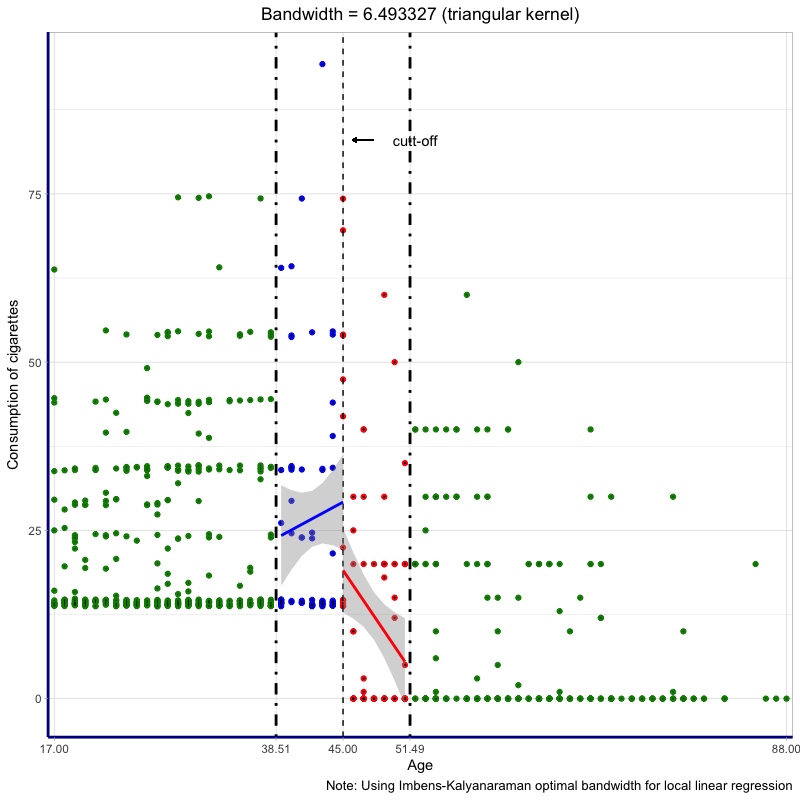
\includegraphics[width=0.99\textwidth]{Rplot13.png}
	\captionof{figure}{Local linear regression (triangular kernel)}
\end{figure}
\begin{figure}[!htb]
	\centering
	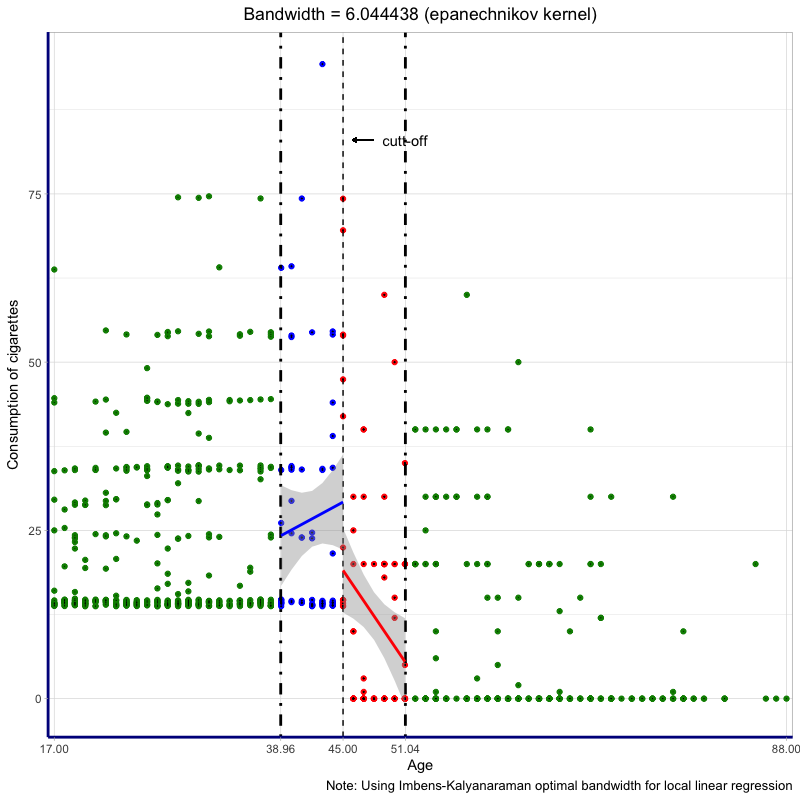
\includegraphics[width=0.99\textwidth]{Rplot14.png}
	\captionof{figure}{Local linear regression (epanechnikov kernel)}
\end{figure}
\begin{figure}[!htb]
	\centering
	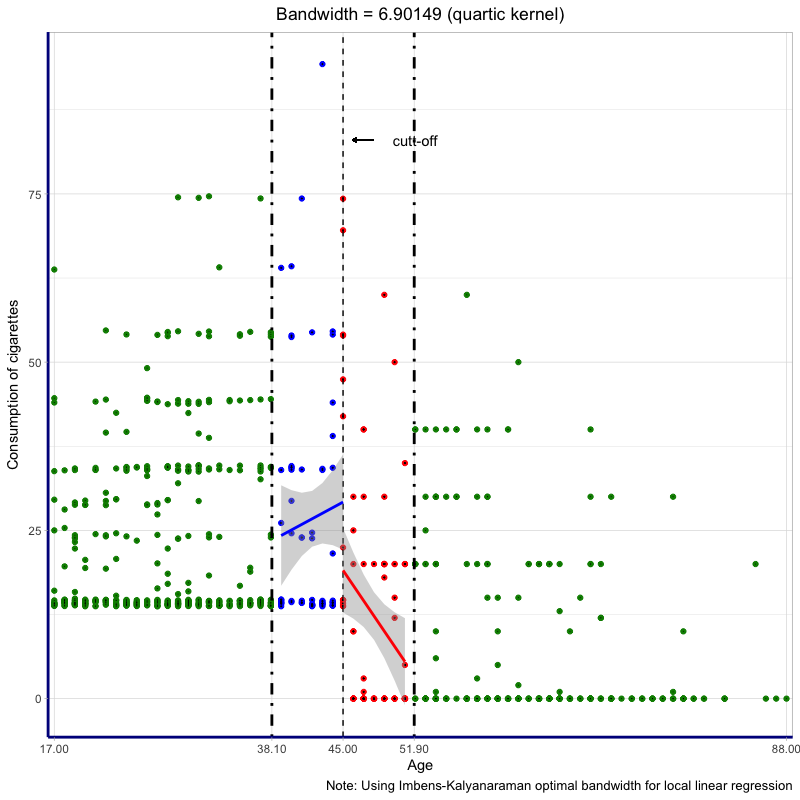
\includegraphics[width=0.99\textwidth]{Rplot15.png}
	\captionof{figure}{Local linear regression (quatric kerne)}
\end{figure}


\end{document}	